% The folded quadrature-point store of the tensor-product elements (Section "What the quadrature can
% see"), drawn for HEX8: along every line of points in direction d the dropped point (index 0) passes
% its m = n = d components to the kept one, so a point stores 45, 39, 33 or 27 numbers, and the
% blocked layout holds 288 per element instead of 360.
\documentclass[border=2pt]{standalone}
% Shared preamble of the format diagrams: colours of the paper's figures (paper_figures.py) and
% the drawing styles.  Each diagram is a standalone document built to a PDF of the text width.
\usepackage{amsmath,amssymb}
\usepackage{tikz}
\usetikzlibrary{arrows.meta,calc,decorations.pathreplacing,patterns,positioning}

\definecolor{cindex}{HTML}{BDBDBD}  % column indices, offsets, row pointers
\definecolor{cvalue}{HTML}{6E6E6E}  % floating-point values (BSR)
\definecolor{cpoint}{HTML}{1B9E77}  % quadrature-point store
\definecolor{celem}{HTML}{1F78B4}   % element matrix
\definecolor{cqbsr}{HTML}{A6761D}   % quantized BSR
\definecolor{cscale}{HTML}{E6AB02}  % scales
\definecolor{cmean}{HTML}{7570B3}   % f32 element mean

\tikzset{
  >={Stealth[length=4pt]},
  grid/.style={draw=black!45, line width=0.25pt},
  frame/.style={draw=black!70, line width=0.5pt},
  title/.style={font=\small\bfseries, anchor=west, inner sep=0pt},
  lab/.style={font=\footnotesize, inner sep=1pt},
  note/.style={font=\scriptsize, text=black!75, inner sep=1pt, execute at begin node={\hyphenpenalty=10000\exhyphenpenalty=10000}},
  num/.style={font=\tiny, inner sep=0pt},
  brace/.style={decorate, decoration={brace, amplitude=3pt, raise=1pt}, line width=0.4pt},
  arr/.style={->, line width=0.5pt, black!70},
  pad/.style={pattern=north east lines, pattern color=black!30},
}

% \cell{x}{y}{w}{h}{fill}: a filled rectangle with a thin outline, lower-left corner at (x,y).
\newcommand{\cell}[5]{\filldraw[fill=#5, grid] (#1,#2) rectangle ++(#3,#4);}
% \blk{x}{y}{s}{fill}: a 3x3 block of side s with its 3x3 entry grid.
\newcommand{\blk}[4]{%
  \filldraw[fill=#4, grid] (#1,#2) rectangle ++(#3,#3);
  \draw[draw=white, line width=0.25pt] (#1,#2) ++(#3/3,0) -- ++(0,#3) ++(#3/3,0) -- ++(0,-#3);
  \draw[draw=white, line width=0.25pt] (#1,#2) ++(0,#3/3) -- ++(#3,0) ++(0,#3/3) -- ++(-#3,0);
  \draw[grid] (#1,#2) rectangle ++(#3,#3);}
% \vthree{x}{y}{fill}: a 3-vector (one node's components) as three small cells, left end at (x,y).
\newcommand{\vthree}[3]{\foreach \k in {0,1,2} \filldraw[fill=#3, grid] (#1+\k*0.14,#2) rectangle ++(0.14,0.14);}
% \op{x}{y}{symbol}: an operation in a small circle.
\newcommand{\op}[3]{\node[circle, draw=black!70, line width=0.4pt, inner sep=0.5pt, minimum size=9pt, font=\tiny] at (#1,#2) {#3};}

\definecolor{cdirA}{HTML}{D95F02}  % m = n = 1
\definecolor{cdirB}{HTML}{E7298A}  % m = n = 2
\definecolor{cdirC}{HTML}{66A61E}  % m = n = 3
\begin{document}
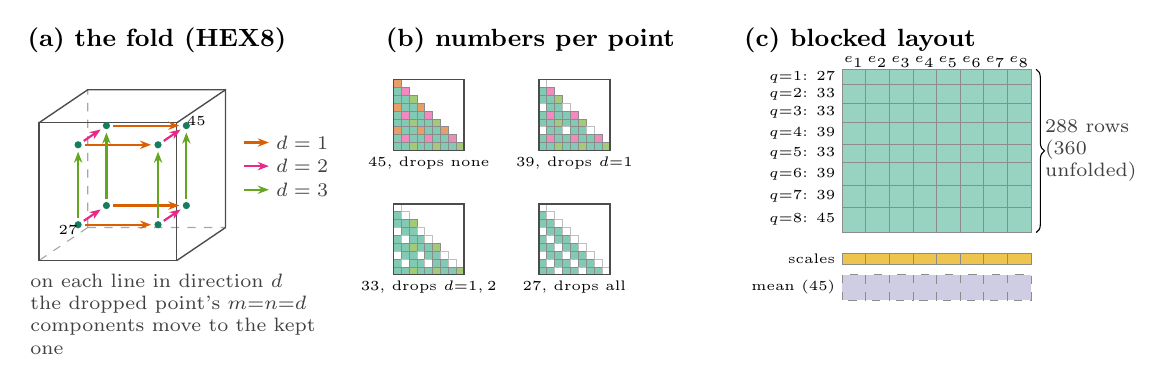
\begin{tikzpicture}
  % ---------------------------------------------------------------- (a) the fold along the lines
  \node[title] at (0, 3.35) {(a) the fold (HEX8)};
  \begin{scope}[shift={(0.15,0.55)}, x={(1.75cm,0cm)}, y={(0.62cm,0.42cm)}, z={(0cm,1.75cm)}]
    % the cube: hidden edges dashed
    \draw[black!35, line width=0.4pt, dashed] (0,1,0) -- (0,0,0) (0,1,0) -- (1,1,0) (0,1,0) -- (0,1,1);
    \draw[frame] (0,0,0) -- (1,0,0) -- (1,0,1) -- (0,0,1) -- cycle;
    \draw[frame] (1,0,0) -- (1,1,0) -- (1,1,1) -- (1,0,1);
    \draw[frame] (0,0,1) -- (0,1,1) -- (1,1,1);
    \def\ga{0.21}\def\gb{0.79}
    % one arrow per line of points, from the dropped point (index 0) to the kept one
    \foreach \u in {\ga,\gb} \foreach \v in {\ga,\gb} {
      \draw[->, cdirA, line width=0.8pt, shorten <=2.5pt, shorten >=2.5pt] (\ga,\u,\v) -- (\gb,\u,\v);
      \draw[->, cdirB, line width=0.8pt, shorten <=2.5pt, shorten >=2.5pt] (\u,\ga,\v) -- (\u,\gb,\v);
      \draw[->, cdirC, line width=0.8pt, shorten <=2.5pt, shorten >=2.5pt] (\u,\v,\ga) -- (\u,\v,\gb);
    }
    \foreach \x in {\ga,\gb} \foreach \y in {\ga,\gb} \foreach \z in {\ga,\gb}
      \fill[cpoint!80!black] (\x,\y,\z) circle (1.3pt);
    \node[num, anchor=north east] at (\ga,\ga,\ga) {$27$};
    \node[num, anchor=south west] at (\gb,\gb,\gb) {$45$};
  \end{scope}
  \node[note, anchor=north west, text width=4.15cm] at (0, 0.42)
    {on each line in direction $d$ the dropped point's $m{=}n{=}d$ components move to the kept one};
  \foreach \c/\l [count=\k from 0] in {cdirA/{$d=1$}, cdirB/{$d=2$}, cdirC/{$d=3$}} {
    \draw[->, \c, line width=0.8pt] (2.75, 2.05-\k*0.3) -- ++(0.32,0);
    \node[note, anchor=west] at (3.12, 2.05-\k*0.3) {\l};
  }

  % ---------------------------------------------------------------- (b) what a point keeps
  \begin{scope}[shift={(4.55,0)}]
    \node[title] at (0, 3.35) {(b) numbers per point};
    \def\t{0.1}
    % \foldmat{x}{y}{mask}{count}: the packed 9x9 tangent (lower triangle, row r = 3i+n, column
    % c = 3k+m); the m = n = d entries in their direction's colour, blank where the point drops d.
    \foreach \mask/\cnt/\lbl [count=\p from 0] in {0/45/{none}, 1/39/{$d{=}1$}, 3/33/{$d{=}1,2$}, 7/27/{all}} {
      \pgfmathsetmacro{\ox}{0.1+mod(\p,2)*1.85}
      \pgfmathsetmacro{\oy}{1.95-floor(\p/2)*1.58}
      \begin{scope}[shift={(\ox,\oy)}]
        \foreach \r in {0,...,8} \foreach \c in {0,...,\r} {
          \pgfmathtruncatemacro{\n}{mod(\r,3)}
          \pgfmathtruncatemacro{\m}{mod(\c,3)}
          \pgfmathtruncatemacro{\dropped}{\n==\m ? mod(floor(\mask/(2^\n)),2) : 0}
          \ifnum\n=\m
            \ifnum\dropped=1
              \draw[grid, draw=black!25] (\c*\t, {(8-\r)*\t}) rectangle ++(\t,\t);
            \else
              \ifcase\n \filldraw[fill=cdirA!60, grid] (\c*\t, {(8-\r)*\t}) rectangle ++(\t,\t);
              \or \filldraw[fill=cdirB!55, grid] (\c*\t, {(8-\r)*\t}) rectangle ++(\t,\t);
              \or \filldraw[fill=cdirC!60, grid] (\c*\t, {(8-\r)*\t}) rectangle ++(\t,\t);
              \fi
            \fi
          \else
            \filldraw[fill=cpoint!55, grid] (\c*\t, {(8-\r)*\t}) rectangle ++(\t,\t);
          \fi
        }
        \draw[frame] (0,0) rectangle (9*\t, 9*\t);
        \node[num, anchor=north] at (4.5*\t, -0.07) {$\cnt$, drops \lbl};
      \end{scope}
    }
  \end{scope}

  % ---------------------------------------------------------------- (c) the folded blocked layout
  \begin{scope}[shift={(10.35,0)}]
    \def\w{0.3}\def\s{0.0072}
    \node[title] at (-1.25, 3.35) {(c) blocked layout};
    \foreach \v in {1,...,8} \node[num, anchor=south] at ({(\v-0.5)*\w}, 3.0) {$e_{\v}$};
    % the points' groups of rows, x fastest: q = 1 (all three dropped) ... q = 8 (none)
    \def\y{2.98}
    \foreach \cnt [count=\q] in {27,33,33,39,33,39,39,45} {
      \pgfmathsetmacro{\hh}{\cnt*\s}
      \pgfmathsetmacro{\yy}{\y-\hh}
      \foreach \v in {0,...,7} {\filldraw[fill=cpoint!45, grid] (\v*\w, \yy) rectangle ++(\w, \hh);}
      \node[num, anchor=east] at (-0.08, \yy+\hh/2) {$q{=}\q$: $\cnt$};
      \xdef\y{\yy}
    }
    \draw[brace] (8*\w+0.03, 2.98) -- (8*\w+0.03, \y) node[midway, right=3pt, note, align=left] {$288$ rows\\($360$\\unfolded)};
    \foreach \v in {0,...,7} {\cell{\v*\w}{0.5}{\w}{0.14}{cscale!70}}
    \node[num, anchor=east] at (-0.08, 0.57) {scales};
    \foreach \v in {0,...,7} {\filldraw[fill=cmean!35, grid, dashed] (\v*\w, 0.05) rectangle ++(\w, 0.32);}
    \node[num, anchor=east] at (-0.08, 0.21) {mean ($45$)};
  \end{scope}
\end{tikzpicture}
\end{document}
